\documentclass{ieeeaccess}
\usepackage{cite}
\usepackage{amsmath,amssymb,amsfonts}
\usepackage{graphicx}
\usepackage{textcomp}
\usepackage{booktabs}
\usepackage{array}
\newcolumntype{L}[1]{>{\raggedright\arraybackslash}p{#1}}
\usepackage{url}
\usepackage[T1]{fontenc}
\def\BibTeX{{\rm B\kern-.05em{\sc i\kern-.025em b}\kern-.08em
    T\kern-.1667em\lower.7ex\hbox{E}\kern-.125emX}}

\begin{document}
\history{Date of publication xxxx 00, 0000, date of current version xxxx 00, 0000.}
\doi{10.1109/ACCESS.2024.0429000}

\title{DamageSAR-Bench: A Leakage-Audited, Building-Level Benchmark of Frozen Foundation Models for SAR Damage Classification on Unseen Disasters}

\author{\uppercase{Thinuka Lehan}\authorrefmark{1} and
\uppercase{Achala Aponsu}\authorrefmark{1}}

\address[1]{Informatics Institute of Technology (IIT), Colombo, Sri Lanka}

\markboth
{Lehan and Aponsu: DamageSAR-Bench: Frozen Foundation Models for SAR Damage Classification on Unseen Disasters}
{Lehan and Aponsu: DamageSAR-Bench: Frozen Foundation Models for SAR Damage Classification on Unseen Disasters}

\corresp{Corresponding author: Thinuka Lehan (e-mail: thinukalehanfyp@gmail.com).}

\begin{abstract}
Building-damage models for synthetic aperture radar (SAR) lose accuracy on unseen disasters, and current evaluations cannot say why: they score pixels or tiles, use outlines drawn on optical images that do not line up with the radar signal, and rarely control for shortcuts. We present DamageSAR-Bench, an open toolkit and benchmark that classifies damage to given building footprints in native single-channel SAR, holds each disaster out in turn, and locks the test events' labels in code until a pre-registered analysis plan is frozen. Frozen encoders are pooled over each footprint, read out by linear probes, compared with image-free and neighbourhood controls, and judged by a pre-set decision table. On the BRIGHT dataset (14 events; 244,976 instance-labelled buildings in 11), the audit finds that in three of six open events the radar signal sits 1.4 to 2.2 encoder patches (7.5 to 17~m) from the optical outlines in a consistent direction, and that more than 80\% of buildings cover fewer than four patches in 5 of 11 events. On five development events, a frozen DINOv3 encoder with a linear probe reaches a building-level area under the receiver operating characteristic curve of 0.50 to 0.85 (mean 0.62), and an ImageNet-supervised encoder does as well or better (mean 0.66). The building's surroundings alone match the outline score, and building size and crowding alone match it in one event and invert in two, which points to evaluation and calibration, not only representation, as causes of failure. One notebook rebuilds every number from public data.
\end{abstract}

\begin{keywords}
Benchmark testing, building damage assessment, domain generalization, foundation models, pre-registration, reproducibility, synthetic aperture radar
\end{keywords}

\titlepgskip=-21pt

\maketitle

% ---------------------------------------------------------------------------------------------------------------
\section{Introduction}
\label{sec:introduction}
\PARstart{A}{fter} an earthquake, explosion or storm, responders need to know which buildings are damaged within hours. Synthetic aperture radar (SAR) images through cloud and at night, so it is often the first imagery available. Deep models now classify building damage from SAR and optical pairs with good accuracy on the disasters they were trained on. On a new disaster they fall short: on BRIGHT, the largest open multimodal benchmark for this task, the event-level mean intersection over union (mIoU) of seven models drops from 47.7--52.3\% under a mixed split to 34.1--39.4\% when the test event is held out~\cite{chen2025bright}. Frozen foundation models show the same pattern at tile level~\cite{shibli2026shortcut}, and building-level results on Sentinel-1 drop when the event is held out~\cite{currie2026transfer}. The 2026 BRIGHT Challenge, whose final test used two unseen 2025 events, was won with a test mean average precision of 0.182 for detection, outlining and classification~\cite{chen2026challenge}.

Why models fail on unseen events is not known, and current evaluations cannot tell. Three explanations compete, and each predicts a different fix:
\begin{enumerate}
\item \emph{Representation.} The features do not encode damage in a way that transfers between disasters.
\item \emph{Evaluation.} The test measures the wrong thing: metrics are pixel- or tile-level, and building outlines drawn on optical images sit metres away from where the side-looking radar records the building. Models may also exploit context rather than the building itself: a recent study found that 73--87\% of intact buildings were called damaged when moved into damaged neighbourhoods~\cite{guo2026neighbourhood}.
\item \emph{Calibration.} Damage prevalence varies from 3\% to 71\% of buildings across the BRIGHT events whose labels we use for development, so a classifier tuned on one mix of events is miscalibrated on the next.
\end{enumerate}
Separating these requires a test bed that is building-level, SAR-only, held out by event, protected against leakage and shortcuts, and statistically honest about how little six or so test events can show. No released tool does all of this.

We make three contributions:
\begin{itemize}
\item \textbf{C1, DamageSAR-Bench:} an open, tested toolkit and benchmark that evaluates frozen encoders on native single-channel SAR at the level of given building footprints, holds each disaster out, enforces a confirmatory-label lock in code until a pre-registered plan is frozen, and reports per-event and event-level results with a decision table fixed in advance.
\item \textbf{C2, projected-footprint pooling:} pooling each building over the region where the radar is expected to see it, rather than over its optical outline. Shifting geographic information system (GIS) footprints for layover is known~\cite{liu2014height,brunner2010earthquake}; what is new is using it inside frozen-encoder pooling and testing it fairly across disasters against matched controls. Whether it helps is decided on the development events at a gate before any confirmatory use.
\item \textbf{C3, label-free recalibration:} adjusting scores to a new event's damage rate without labels, by expectation--maximization (EM)~\cite{saerens2002adjusting} and black-box shift estimation (BBSE)~\cite{lipton2018bbse}, with an explicit abstain rule. It powers a new-event mode that estimates how many supplied footprints are damaged, or reports that the estimate is unreliable.
\end{itemize}

To our knowledge, no published evaluation combines building-level units, native single-channel very-high-resolution (VHR) SAR, event-held-out testing, image-free and neighbourhood controls, label-free prevalence estimation and a pre-registered, code-enforced test set (Table~\ref{tab:related}). The closest work, a shortcut audit of geospatial foundation models~\cite{shibli2026shortcut}, evaluates tiles and copies SAR into three channels; its authors name building-level evaluation on native sensor inputs as future work.

This paper reports C1 in full, together with the development-event evidence that shapes C2 and C3: the data audit, the first benchmark, and its controls. We do not propose a new network, and we do not detect buildings: footprints are given. The aim is to find out which models can be trusted on the next disaster, and why the others fail.

% ---------------------------------------------------------------------------------------------------------------
\section{Related Work}
\label{sec:related}

\subsection{Building-Damage Benchmarks Under Event Shift}
Classical SAR damage mapping compares pre- and post-event intensity or interferometric coherence~\cite{matsuoka2004sar,plank2014rapid}; a review of SAR-based building-damage methods is given in~\cite{ge2020review}, and deep networks have since been trained on optical--SAR pairs from several disasters~\cite{adriano2021multimodal}. xBD made multi-hazard building-damage assessment from pre- and post-event optical pairs a standard task~\cite{gupta2019xbd}. BRIGHT~\cite{chen2025bright} added VHR SAR: it pairs pre-event optical images with post-event SAR at 0.3--1~m over 14 events and reports both a mixed split and an event-held-out split. Its authors observe that choosing models on source-event validation data is far from the best achievable choice, and ask for selection methods that need no target labels. The 2026 BRIGHT Challenge~\cite{chen2026challenge} extended the data to instance labels for about 291,000 buildings in 16 events; on the two unseen final-phase events, scores fell sharply and the team ranking changed substantially. At 10~m resolution the same pattern holds: Sentinel-1/2 models trained on xBD-S12 lose accuracy on unseen disasters~\cite{dietrich2026copernicus}, and a study of 205,731 buildings across 11 disasters found that holding the event out cut median macro-F1 from 0.68 to 0.54~\cite{currie2026transfer}. A recent review finds that the task is defined inconsistently across the literature and that generalization to unseen events remains open~\cite{cioppa2026revisiting}. None of these evaluates given building footprints in native VHR SAR with frozen encoders and event-level uncertainty.

\subsection{Frozen Foundation-Model Embeddings}
Vision Transformers (ViT)~\cite{dosovitskiy2021vit} trained by self-supervision, such as DINOv2~\cite{oquab2024dinov2} and DINOv3~\cite{simeoni2026dinov3}, give general features that a linear read-out can use. HASTE~\cite{robinson2026haste} pools frozen embeddings over each footprint and fits a per-event logistic regression from a handful of labels, on optical imagery. Closest to our work, Shibli \emph{et al.}~\cite{shibli2026shortcut} audit four geospatial foundation models on xView2 and BRIGHT: holding out the event lowers balanced accuracy on BRIGHT from 0.818 to 0.568, and a one-number building-count baseline reaches 0.653. Their analysis is at tile level, with the SAR band copied into three channels. We work at building level, on native single-channel SAR, and add the controls at that level. SAR-specific foundation models such as CrossEarth-SAR~\cite{ye2026crossearth} target segmentation across sensors and regions; none has been evaluated on building damage.

\subsection{Shortcuts and Leakage}
Shortcut learning, where a model uses a cue that predicts the label in the training data but not in deployment, is well documented~\cite{geirhos2020shortcut}, and data leakage is a common cause of irreproducible results in machine-learning-based science~\cite{kapoor2023leakage}. Spatially structured data need blocked rather than random validation~\cite{roberts2017cv}, and pre-registering the analysis before seeing the outcome separates testing a hypothesis from generating one~\cite{nosek2018prereg}; both are rare in remote sensing. For damage mapping, Guo \emph{et al.}~\cite{guo2026neighbourhood} show that models miss a third to half of isolated damaged buildings and, in non-flood events, call 73--87\% of intact buildings damaged once they are moved into a damaged neighbourhood. DamageSAR-Bench builds these concerns into the protocol: image-free and building-size controls, a neighbourhood control, and a code-level lock on the confirmatory events' labels.

\subsection{SAR Geometry and Building Footprints}
A side-looking radar records a building displaced towards the sensor (layover), by an amount that grows with height, and casts a shadow behind it. Liu \emph{et al.}~\cite{liu2014height} shift GIS footprints towards the sensor to estimate building height from TerraSAR-X, and Brunner \emph{et al.}~\cite{brunner2010earthquake} predict each building's expected post-event SAR signature from optical-derived 3-D parameters and classify it by its similarity to the observed image. C2 takes this geometric idea into frozen-encoder pooling and tests it across disasters against matched controls.

\subsection{Prior Shift and Recalibration}
When only the class balance changes between source and target, a classifier's posteriors can be corrected without target labels, by EM~\cite{saerens2002adjusting} or by BBSE~\cite{lipton2018bbse}. EM combined with bias-corrected calibration is a strong baseline among such methods~\cite{alexandari2020bcts}. The BRIGHT Challenge winner gained much of its final score from per-scene threshold recalibration and pseudo-labels~\cite{chen2026challenge}, an ad hoc form of the same idea. C3 applies these estimators to building-level scores, and adds a rule to abstain when the estimate is unreliable.

\subsection{Positioning}
Table~\ref{tab:related} sets the closest studies against DamageSAR-Bench on the elements that the three explanations in Section~\ref{sec:introduction} require. Each earlier study covers some of them; none covers all.

\begin{table*}[t]
\centering
\caption{Closest work. \checkmark{} = a main element of the study; -- = not a main element.}
\label{tab:related}
\footnotesize
\setlength{\tabcolsep}{3pt}\begin{tabular}{@{}L{2.3cm}L{2.0cm}L{2.9cm}L{2.1cm}L{2.3cm}L{2.3cm}L{1.9cm}@{}}
\toprule
Study & Unit & Post-event input & Unseen-event test & Shortcut controls & Label-free prevalence & Pre-registered test \\
\midrule
BRIGHT~\cite{chen2025bright} & Pixel & VHR SAR (+ pre-event optical) & \checkmark & -- & -- & -- \\
BRIGHT Challenge~\cite{chen2026challenge} & Instance (detect + classify) & VHR SAR (+ pre-event optical) & \checkmark{} (2 events) & -- & Ad hoc per-scene thresholds & -- \\
Shibli \emph{et al.}~\cite{shibli2026shortcut} & Tile & VHR SAR copied to 3 channels (+ optical) & \checkmark & \checkmark{} (image-free, count) & -- & -- \\
Currie and Reinke~\cite{currie2026transfer} & Building & Sentinel-1, 10~m & \checkmark & -- & -- & -- \\
Guo \emph{et al.}~\cite{guo2026neighbourhood} & Building & VHR optical; optical--SAR check & Partly & \checkmark{} (neighbourhood) & -- & -- \\
HASTE~\cite{robinson2026haste} & Building & VHR optical & Per event, with labels & -- & -- & -- \\
\midrule
\textbf{DamageSAR-Bench} & \textbf{Building (given footprint)} & \textbf{Native single-channel VHR SAR} & \textbf{\checkmark{} (leave-one-event-out)} & \textbf{\checkmark{} (image-free, neighbourhood)} & \textbf{\checkmark{} (EM/BBSE + abstain)} & \textbf{\checkmark{} (code-level lock)} \\
\bottomrule
\end{tabular}
\end{table*}

% ---------------------------------------------------------------------------------------------------------------
\section{Data}
\label{sec:data}

\subsection{BRIGHT}
We use BRIGHT~\cite{chen2025bright}: 4,246 post-event SAR tiles of $1024\times1024$ pixels over 14 events and five hazard types, with pixel labels (intact, damaged, destroyed) and, for 11 events, building instance polygons drawn on the pre-event optical image (Zenodo record 19216381). Ground resolution is 0.2--0.6~m; four events are stored in geographic coordinates (EPSG:4326) and one in Web Mercator (EPSG:3857), so all areas are computed in true ground metres. The reported optical--SAR co-registration error is about 1.02 pixels root-mean-square~\cite{chen2025bright}.

\subsection{Event Roles}
Each event has one fixed role (Table~\ref{tab:roles}). Confirmatory events are the test of the pre-registered claims; their labels are refused by the code until the analysis plan is frozen on 10 January 2027. Development events are used to design and tune everything. Secondary events add breadth to a supporting random-effects estimate. Ukraine has no instance labels; it uses open footprints only if they agree with the label raster on at least 80\% of buildings in the development events, and otherwise moves to the secondary set, leaving five confirmatory events.

\begin{table}[t]
\centering
\caption{Event roles.}
\label{tab:roles}
\footnotesize
\begin{tabular}{@{}L{1.55cm}L{3.9cm}L{1.95cm}@{}}
\toprule
Role & Events (hazard) & Building units \\
\midrule
Confirmatory (6) & Haiti, T\"urkiye, Morocco, Noto (earthquake); Bata (explosion); Ukraine (conflict) & Instance polygons; Ukraine by a fallback rule \\
Development (5) & Beirut (explosion); La Palma, Congo (volcano); Hawaii (wildfire); Libya (flood) & Instance polygons \\
Secondary (3) & Marshall (wildfire); Mexico, Myanmar (storm) & Marshall only \\
\bottomrule
\end{tabular}
\end{table}

\subsection{Building Table and No-Data Rule}
One unit is one instance polygon, labelled damaged-or-destroyed (positive) or intact by its class in the instance file. Tiles with at least 95\% SAR no-data (value 0) are excluded (20 tiles), and so are buildings whose footprint is at least half no-data. The 11 labelled events hold 244,976 buildings; 242,842 remain (828 excluded for building no-data, 753 for tile no-data, 553 empty footprints). For every unlocked event the instance class matches the majority label-raster class inside the polygon for 99.9--100\% of buildings. One detail matters to anyone reusing the labels: the \texttt{area} field in BRIGHT's instance files is the bounding-box area (width $\times$ height), not the polygon area, for every building; our table stores both.

Prevalence differs widely: among the development and secondary events, damaged or destroyed buildings range from 3.1\% (Beirut) to 71.1\% (Hawaii) of an event's kept buildings. The positive counts are Beirut 653 (25 destroyed), Libya 3,346, Congo 1,505, Hawaii 2,511, La Palma 5,596 and Marshall 696. Confirmatory class counts stay hidden until the freeze.

% ---------------------------------------------------------------------------------------------------------------
\section{Method}
\label{sec:method}

\subsection{Pipeline}
DamageSAR-Bench is a Python package with a command-line interface. Each stage reads typed, versioned inputs and writes resumable outputs, and every hand-over checks that no confirmatory label passes before the freeze date (Fig.~\ref{fig:pipeline}).

\begin{figure}[t]
\centering
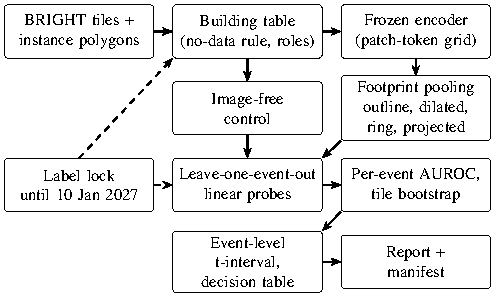
\includegraphics[width=\columnwidth]{figures/fig_pipeline.pdf}
\caption{Pipeline. Building table (\texttt{bench buildings}), feature extraction with footprint pooling (\texttt{bench extract}, sharded and resumable), leave-one-event-out probes, statistics and report (\texttt{bench run}, \texttt{bench report}). Dashed arrows: the confirmatory-label lock, checked at every hand-over.}
\label{fig:pipeline}
\end{figure}

\subsection{Encoders and Input}
The core encoders are an ImageNet-supervised ViT-B/16, DINOv2 ViT-B/14~\cite{oquab2024dinov2} and DINOv3 ViT-B/16 with web-scale (LVD) pre-training~\cite{simeoni2026dinov3}; all are frozen. Single-channel SAR intensity is copied into three channels and normalized with the ImageNet statistics. A ViT/16 patch token covers 4.8--9.6~m of ground at BRIGHT's native resolutions, so many buildings cover only a few tokens (Section~\ref{sec:res-size}). We therefore compare native resolution with resampling every tile to a common 0.3~m before encoding.

\subsection{Footprint Pooling}
Let $\mathbf{z}_t\in\mathbb{R}^{D}$ be the feature of patch token $t$ in a tile, $P_b$ the region of building $b$, and $|P_b\cap t|$ the ground area of $P_b$ inside token $t$. The building's vector is the area-weighted mean
\begin{equation}
\mathbf{x}_b=\frac{\sum_{t}|P_b\cap t|\,\mathbf{z}_t}{\sum_{t}|P_b\cap t|}.
\label{eq:pool}
\end{equation}
Three regions are used. \emph{Outline} pooling takes $P_b$ as the polygon; \emph{dilated} pooling grows it by 3~m, measured in ground metres per axis so that tiles stored in degrees are handled correctly; and the \emph{ring} (neighbourhood control) takes the band up to 10~m outside the polygon, excluding every token that contains any building pixel, and falls back to the eight tokens around the building's token if no token remains (this fallback was never needed on the development events). Buildings smaller than one pixel take the token at their centre and are flagged.

\subsection{Probes and Metric}
For each held-out event $e$, an L2-regularized logistic regression is trained on the buildings of the other events, $\mathcal{T}_e$:
\begin{equation}
\min_{\mathbf{w},c}\;\frac{1}{2}\|\mathbf{w}\|^2+C\sum_{b\in\mathcal{T}_e}\omega_{y_b}\log\!\left(1+e^{-\tilde y_b(\mathbf{w}^{\top}\tilde{\mathbf{x}}_b+c)}\right),
\label{eq:probe}
\end{equation}
where $\tilde{\mathbf{x}}_b$ is $\mathbf{x}_b$ standardized with statistics from $\mathcal{T}_e$ only, $y_b\in\{0,1\}$ marks damaged-or-destroyed, $\tilde y_b=2y_b-1$, $\omega_{y}$ are balanced class weights (inversely proportional to class frequency in $\mathcal{T}_e$) and $C=1$, fixed and never tuned on the held-out event. Before the freeze, probes train on development and secondary events only. The metric is the building-level area under the receiver operating characteristic curve (AUROC) of the probe's scores $s_b$ on event $e$, with $n_1$ positive and $n_0$ negative buildings:
\begin{equation}
\mathrm{AUROC}_e=\frac{1}{n_1n_0}\sum_{i:\,y_i=1}\sum_{j:\,y_j=0}\Big[\mathbb{1}(s_i>s_j)+\tfrac{1}{2}\mathbb{1}(s_i=s_j)\Big].
\label{eq:auroc}
\end{equation}
AUROC is 0.5 for a random ranking and does not depend on prevalence. Its uncertainty within one event comes from a bootstrap that resamples tiles, not buildings (2,000 replicates, seed 0), because buildings in one tile are not independent.

\subsection{C2: Projected-Footprint Pooling}
In a side-looking SAR image a building of height $h$ appears displaced towards the sensor by about
\begin{equation}
\Delta_{\mathrm{lay}}=h\cot\theta,
\label{eq:layover}
\end{equation}
where $\theta$ is the incidence angle from vertical, with a shadow of about $h\tan\theta$ behind it. C2 moves the pooling region of~\eqref{eq:pool} by $\Delta_{\mathrm{lay}}$ towards the sensor, along the scene's look direction, where viewing geometry is known; elsewhere dilated pooling is used instead of a guess. C2 must beat three controls of matched size: dilated pooling, a randomly directed shift, and a shift across the look direction.

\subsection{C3: Label-Free Recalibration}
The probe's scores on a new event are adjusted to that event's estimated damage prevalence by EM~\cite{saerens2002adjusting} or BBSE~\cite{lipton2018bbse}, without its labels. The estimate gives a damaged-building count for the supplied footprints, or an abstention when the estimate is unstable.

\subsection{Controls}
Every benchmark run reports two controls. The \emph{image-free} control uses no pixels: a probe of the same form~\eqref{eq:probe} on four geometry features per building (log footprint area, log number of buildings in its tile, log number of buildings within 50~m, and log distance to the nearest building). The \emph{neighbourhood} control is the same encoder pooled over the ring, which sees the surroundings but not the building. A model that does not beat its controls is not credited with recognizing damage.

% ---------------------------------------------------------------------------------------------------------------
\section{Experimental Setup and Pre-Registration}
\label{sec:setup}

\subsection{Research Questions}
\begin{itemize}
\item \textbf{RQ1} (primary). Does a modern self-supervised encoder (DINOv3) classify damage to given footprints on an unseen disaster better than an ImageNet-supervised ViT-B?
\item \textbf{RQ2} (primary, only if Gate~1 passes). Does projected-footprint pooling beat outline pooling?
\item \textbf{RQ3} (exploratory). How accurately can a new event's damage prevalence be estimated without labels, and how often must the estimate abstain?
\item \textbf{RQ4} (exploratory). How much of each model's score do the image-free and neighbourhood controls already reach?
\end{itemize}

\subsection{Statistics}
The event is the unit of inference, because buildings and tiles within one disaster are not independent; this follows the practice of comparing classifiers by their per-data-set results~\cite{demsar2006comparisons}. For a comparison of setting $A$ with setting $B$ over $n$ events, the per-event gain is $g_e=\mathrm{AUROC}_e^{A}-\mathrm{AUROC}_e^{B}$, and
\begin{equation}
\bar g\pm t_{1-\alpha/2,\,n-1}\,\frac{s_g}{\sqrt{n}},
\label{eq:tint}
\end{equation}
where $\bar g$ and $s_g$ are the mean and standard deviation of the gains and $t_{1-\alpha/2,n-1}$ is the Student-$t$ quantile ($\alpha=0.05$, or $0.025$ per claim if a Bonferroni split is adopted). With lower and upper ends $\ell$ and $u$ of~\eqref{eq:tint} and the smallest worthwhile gain $\delta=0.02$, the verdict is the first that applies of: (i) $\ell>0$ and $\bar g\ge\delta$: a worthwhile gain; (ii) $\ell>0$ and $\bar g<\delta$: a small positive effect, below worthwhile; (iii) $\ell\le0$ and $u<\delta$: not a worthwhile gain; (iv) otherwise: inconclusive.

An exact sign-flip test and a Hartung--Knapp random-effects estimate~\cite{hartung2001knapp} over the secondary set are reported as supporting evidence only. With six events, the minimum detectable mean gain at two-sided 5\% and 80\% power is $1.43\,s_g$ (1.68\,$s_g$ with five), solved with the noncentral $t$ distribution; the smallest attainable sign-flip $p$ is $2/64$ ($2/32$). The statistics code is tested against hand-worked values, printed tables, scikit-learn and statsmodels.

\subsection{Gates and What Was Seen Before the Freeze}
Gate~1 (18 December 2026, development events only) decides whether C2 proceeds to RQ2: its mean AUROC gain over outline pooling must be at least $+0.02$ and it must beat the random-shift control. C3 passes if its relative prevalence error is at most 50\% on at least four of five development events and lower than a training-average baseline.

An audit on 31 October 2026 looked at confirmatory events in four limited ways: class and instance counts, footprint-to-SAR offsets, raw-signal AUROC and a building-count AUROC. No encoder features were computed and no setting was chosen from them. The offsets motivated C2, which is therefore designed and gated on development events only. This disclosure is part of the pre-registration.

\subsection{Implementation and Compute}
The toolkit is written in Python (PyTorch 2.14, Transformers 5.22, scikit-learn 1.6, rasterio 1.5) and has more than 220 unit tests. All runs used one NVIDIA T4 GPU on Google Colab with 12.7~GB of system memory. DINOv3 ViT-B/16 encodes a 1024-pixel tile in half precision at about 10.5 tiles/s with 0.36~GB of GPU memory; with file reading and pooling, the 1,026 development and secondary tiles took 501--506~s for DINOv3 and 783~s for the ImageNet ViT-B at native resolution, and 738~s for DINOv3 at 0.3~m.

% ---------------------------------------------------------------------------------------------------------------
\section{Results}
\label{sec:results}
All numbers in this section come from development and secondary events, or are counts and geometry that use no confirmatory labels. They are descriptive or exploratory; no confirmatory claim is made.

\subsection{Data Audit and Reproduction}
The toolkit's data checks reproduced an earlier independent validation exactly in a second computing account: 4,246 tiles, no unreadable tiles, the same per-event tile counts and the same 20 no-data exclusions. Every number in this paper is listed with its source run and tolerance in the repository, and one notebook rebuilds them from the public data in a fresh session and checks each; run in a fresh session, it reproduced every checked value, with counts identical and the largest AUROC difference 0.002 (see Data and Code Availability).

To measure how far the SAR signal sits from the optical footprints, each tile's footprint mask is cross-correlated with its SAR image at quarter resolution within $\pm40$~m. A shift counts as clear when its correlation peak stands at least 3 standard deviations above the search window, and as real when it beats the same footprints matched against three other tiles of the event (a permutation null). Table~\ref{tab:offsets} gives the result. In Congo, Libya and Beirut the signal sits 7.5--17~m away, 1.4--2.2 tokens, in a consistent direction (mean resultant length $R=0.77$--$0.86$), and the shift beats the null in 33--73\% of tiles. In Hawaii and Marshall it does not (12.5\% and 0\% of tiles; under one token): there the outlines already line up. La Palma's shift is weak and has no consistent direction. Because scene co-registration error is about one pixel~\cite{chen2025bright}, whole-scene misregistration is an unlikely sole cause; whether the offset is layover, local misalignment or both is tested in C2.

\begin{table}[t]
\centering
\caption{Footprint-to-SAR offset per tile (development and secondary events). Median over tiles with a clear peak; $R$ = consistency of direction (1 = all tiles shift the same way).}
\label{tab:offsets}
\footnotesize
\begin{tabular}{@{}lrrrrrr@{}}
\toprule
Event & Tiles & Clear & Median & Tokens & Beats null & $R$ \\
\midrule
Congo & 92 & 89\% & 7.5~m & 1.41 & 73\% & 0.84 \\
Libya & 98 & 38\% & 11.3~m & 2.02 & 48\% & 0.86 \\
Beirut & 111 & 15\% & 17.2~m & 2.15 & 33\% & 0.77 \\
La Palma & 603 & 27\% & 11.1~m & 2.30 & 29\% & 0.36 \\
Hawaii & 56 & 80\% & 4.2~m & 0.75 & 12.5\% & 0.52 \\
Marshall & 66 & 92\% & 2.4~m & 0.25 & 0\% & 0.63 \\
\bottomrule
\end{tabular}
\end{table}

\subsection{Buildings Are Small Relative to Encoder Tokens}
\label{sec:res-size}
Table~\ref{tab:tokens} gives, for each labelled event, the share of buildings that cover fewer than four ViT/16 tokens at native resolution and after resampling to 0.3~m. At native resolution, more than a quarter of buildings in every event cover fewer than four tokens, and in Congo, Marshall, Haiti, Noto and Bata more than 80\% do. Resampling to 0.3~m cuts the share by 1.6--4$\times$ for the coarser events (Beirut 41.9 to 13.3\%, Marshall 91.4 to 22.6\%) and changes little where the native resolution is already near 0.3~m. In Congo and La Palma, 70--92\% of buildings stay under four tokens even at 0.3~m: a building's vector is mostly its surroundings. This limits what any footprint-pooling method, including C2, can do there, and raises the risk of the neighbourhood shortcut~\cite{guo2026neighbourhood}.

\begin{table}[t]
\centering
\caption{Share of kept buildings covering fewer than four ViT/16 tokens (\%). Geometry only; no labels are used.}
\label{tab:tokens}
\footnotesize
\begin{tabular}{@{}llrr@{}}
\toprule
Event & Role & Native & At 0.3~m \\
\midrule
Beirut & development & 41.9 & 13.3 \\
Congo & development & 95.5 & 91.8 \\
Hawaii & development & 32.4 & 24.5 \\
La Palma & development & 69.8 & 69.8 \\
Libya & development & 28.4 & 20.4 \\
Marshall & secondary & 91.4 & 22.6 \\
Bata & confirmatory & 84.0 & 30.7 \\
Haiti & confirmatory & 88.8 & 53.9 \\
Morocco & confirmatory & 33.2 & 32.1 \\
Noto & confirmatory & 90.6 & 51.4 \\
T\"urkiye & confirmatory & 26.0 & 22.4 \\
\bottomrule
\end{tabular}
\end{table}

\subsection{Benchmark v0 on Development Events}
We ran DINOv3 ViT-B/16 (frozen) at native resolution and resampled to 0.3~m, with outline and 3~m dilated pooling, and held out each development event in turn; probes trained on the other development events and Marshall (58,094--84,354 training buildings per fold; every probe converged in at most 175 iterations). Table~\ref{tab:auroc} gives the per-event AUROC and Table~\ref{tab:cmp} the event-level comparisons.

\begin{table*}[t]
\centering
\caption{Building-level AUROC (damaged-or-destroyed vs.\ intact) on each held-out development event, frozen DINOv3 ViT-B/16 with a linear probe. Brackets: 95\% tile-cluster bootstrap interval for native outline pooling.}
\label{tab:auroc}
\footnotesize
\begin{tabular}{@{}lrcccc@{}}
\toprule
Event (hazard) & Buildings (positive) & Native, outline & Native, dilated 3~m & 0.3~m, outline & 0.3~m, dilated 3~m \\
\midrule
Beirut (explosion) & 20,859 (653) & 0.646 [0.381, 0.873] & 0.651 & 0.531 & 0.543 \\
Congo (volcano) & 16,531 (1,505) & 0.849 [0.792, 0.897] & 0.853 & 0.762 & 0.774 \\
Hawaii (wildfire) & 3,532 (2,511) & 0.504 [0.403, 0.607] & 0.501 & 0.576 & 0.566 \\
La Palma (volcano) & 29,792 (5,596) & 0.604 [0.548, 0.658] & 0.605 & 0.598 & 0.598 \\
Libya (flood) & 9,573 (3,346) & 0.498 [0.387, 0.605] & 0.478 & 0.486 & 0.497 \\
\midrule
Mean of 5 events & & 0.620 & 0.618 & 0.591 & 0.596 \\
\bottomrule
\end{tabular}
\end{table*}

\begin{table}[t]
\centering
\caption{Event-level comparisons for DINOv3 (5 events, t-interval with 4 degrees of freedom, 95\%). SD = standard deviation of the per-event gains.}
\label{tab:cmp}
\footnotesize
\resizebox{\columnwidth}{!}{%
\begin{tabular}{@{}lrcrl@{}}
\toprule
Comparison & Gain & 95\% interval & SD & Verdict \\
\midrule
0.3~m vs.\ native, outline & $-0.030$ & [$-0.122$, $+0.062$] & 0.074 & Inconclusive \\
0.3~m vs.\ native, dilated & $-0.022$ & [$-0.110$, $+0.066$] & 0.071 & Inconclusive \\
Dilated vs.\ outline, native & $-0.003$ & [$-0.015$, $+0.010$] & 0.010 & Not worthwhile \\
Dilated vs.\ outline, 0.3~m & $+0.005$ & [$-0.008$, $+0.018$] & 0.010 & Not worthwhile \\
\bottomrule
\end{tabular}}
\end{table}

Three observations follow. First, frozen features transfer very unevenly: Congo reaches 0.85, while Hawaii (wildfire) and Libya (flood) stay at chance. A single mean across events hides this, which is why the benchmark reports every event. Second, resampling to 0.3~m does not help on average; it costs 0.08--0.12 AUROC in Beirut and Congo and gains 0.06--0.07 in Hawaii, so the resolution choice interacts with the event, and native resolution is kept, as it is also cheaper. Third, growing the footprint by 3~m changes AUROC by at most 0.02 in any event, and its gains vary little between events (SD 0.010). For a pooling comparison of this kind, the pre-registered pilot rule ($s_g\le0.020$) is met, and with six events the minimum detectable mean gain would be about $1.43\times0.010\approx0.014$ AUROC, below $\delta$. The C2 test is therefore adequately powered if its gains vary as little as dilation's; the resolution comparison, with SD 0.07, would not be.

\subsection{Controls and the ImageNet Baseline}
\label{sec:controls}
Table~\ref{tab:controls} and Fig.~\ref{fig:auroc} add the two controls and the ImageNet-supervised ViT-B/16 at native resolution, under the same probes and folds (30 probes, all converged in at most 250 iterations), and Table~\ref{tab:cmp2} gives the event-level comparisons. All six comparisons are inconclusive with five events; what they show is in the per-event pattern.

\begin{figure}[t]
\centering
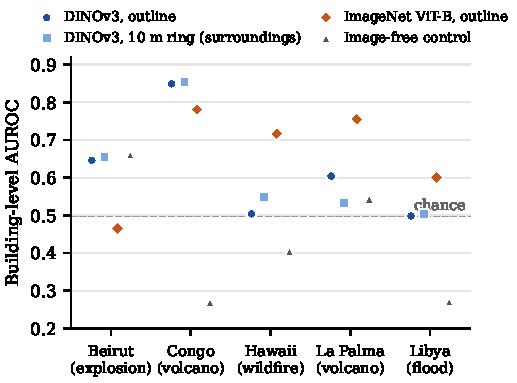
\includegraphics[width=\columnwidth]{figures/fig_auroc.pdf}
\caption{Building-level AUROC per held-out development event for frozen DINOv3 pooled over the outline and over the 10~m surroundings only, the ImageNet-supervised ViT-B (outline), and the image-free control. Dashed line: chance.}
\label{fig:auroc}
\end{figure}

\begin{table*}[t]
\centering
\caption{Building-level AUROC with controls and the ImageNet baseline (native resolution, held-out development events).}
\label{tab:controls}
\footnotesize
\begin{tabular}{@{}lcccccc@{}}
\toprule
Setting & Beirut & Congo & Hawaii & La Palma & Libya & Mean \\
\midrule
DINOv3, outline & 0.646 & 0.849 & 0.504 & 0.604 & 0.498 & 0.620 \\
DINOv3, 10~m ring (surroundings only) & 0.654 & 0.853 & 0.549 & 0.533 & 0.503 & 0.618 \\
ImageNet ViT-B, outline & 0.465 & 0.781 & 0.716 & 0.755 & 0.600 & 0.663 \\
ImageNet ViT-B, dilated 3~m & 0.451 & 0.821 & 0.710 & 0.780 & 0.603 & 0.673 \\
ImageNet ViT-B, 10~m ring (surroundings only) & 0.385 & 0.697 & 0.727 & 0.815 & 0.542 & 0.633 \\
Image-free control (size and crowding) & 0.661 & 0.269 & 0.405 & 0.544 & 0.272 & 0.430 \\
\bottomrule
\end{tabular}
\end{table*}

\begin{table}[t]
\centering
\caption{Event-level comparisons with controls and the ImageNet baseline (5 events, 95\% t-interval). All verdicts: inconclusive.}
\label{tab:cmp2}
\footnotesize
\begin{tabular}{@{}lrcr@{}}
\toprule
Comparison & Gain & 95\% interval & SD \\
\midrule
DINOv3 vs.\ ImageNet (outline) & $-0.043$ & [$-0.246$, $+0.159$] & 0.163 \\
Outline vs.\ ring, DINOv3 & $+0.002$ & [$-0.051$, $+0.054$] & 0.042 \\
Outline vs.\ ring, ImageNet & $+0.030$ & [$-0.048$, $+0.109$] & 0.063 \\
DINOv3 vs.\ image-free & $+0.190$ & [$-0.102$, $+0.482$] & 0.235 \\
ImageNet vs.\ image-free & $+0.234$ & [$-0.094$, $+0.561$] & 0.264 \\
Dilated vs.\ outline, ImageNet & $+0.009$ & [$-0.018$, $+0.037$] & 0.022 \\
\bottomrule
\end{tabular}
\end{table}

Three findings stand out. First, the newer self-supervised encoder is not better here: the ImageNet ViT-B reaches a higher mean AUROC (0.663 against 0.620) and is ahead on three of five events (Hawaii by 0.21, La Palma by 0.15, Libya by 0.10), while DINOv3 is ahead in Beirut (0.18) and Congo (0.07). The hazards on which each encoder leads differ, so the RQ1 comparison is unlikely to be settled by a uniform gain.

Second, the building's own tokens add no measurable information over its surroundings. DINOv3 pooled over the 10~m ring, which never touches a building token, scores as well as outline pooling in every event but La Palma (mean 0.618 against 0.620), and in Congo it matches the outline score (0.853 against 0.849). Congo's high AUROC therefore reflects where damaged buildings are, inside the lava-affected area, rather than what they look like in SAR, as suspected from its small buildings (Table~\ref{tab:tokens}). With ImageNet features the outline is ahead of the ring in Beirut, Congo and Libya by 0.06--0.08, but behind it in Hawaii and La Palma.

Third, the image-free control behaves very differently from event to event. In Beirut, building size and crowding alone reach 0.661, as high as either encoder, so the encoders' Beirut scores are not evidence that they see damage. In Congo and Libya the control falls far below chance (0.269 and 0.272): the relationship between building geometry and damage that the probe learns on the other events is reversed on these. This is a shortcut that does not transfer, of the kind that a mixed split rewards and an event-held-out split exposes.

\subsection{Confirmatory Test}
The six confirmatory events remain locked. After the analysis plan is frozen on 10 January 2027, RQ1 and, if Gate~1 passes, RQ2 are run once on them with the event-level intervals and the decision table of Section~\ref{sec:setup}; RQ3 and RQ4 are reported as exploratory.

% ---------------------------------------------------------------------------------------------------------------
\section{Discussion and Limitations}
\label{sec:discussion}

\textbf{What the results say about the three explanations.} The evidence bears on each explanation of Section~\ref{sec:introduction} without settling any. \emph{Representation:} frozen features separate damaged from intact buildings clearly in some events and not at all in others, and which encoder does better depends on the event; for DINOv3 in wildfire and flood, the features do not carry damage in a form a linear probe can transfer. \emph{Evaluation:} outlines are offset from the SAR signal by one to two tokens in three of six open events (Table~\ref{tab:offsets}); most buildings in several events are smaller than a few tokens; and the surroundings alone reproduce the outline score. A building-level score from frozen features at native resolution is therefore largely a score of the building's neighbourhood. \emph{Calibration:} prevalence ranges from 3\% to 71\% across the development and secondary events, and the image-free control shows that even the direction of the geometry--damage relationship changes between events. AUROC does not depend on prevalence, so the prevalence effect itself will show in threshold-based metrics and in C3.

\textbf{What the design can and cannot show.} With five or six events, only large and consistent gains can be detected ($1.43\,s_g$ with six). Every comparison so far is inconclusive, and the per-event gains between the two encoders have an SD of 0.16; we therefore treat an inconclusive verdict as a real and reportable outcome, report the estimate and its interval whatever the verdict, and keep secondary and exploratory analyses separate from the primary claims.

\textbf{Can C2 matter?} Dilating footprints by 3~m, about half a token, changed AUROC by at most 0.02 in any event, so a shift smaller than about one token barely changes a building's vector. Table~\ref{tab:offsets} shows no offset beyond the permutation null in Hawaii or Marshall, and only a weak, scattered one in La Palma, so C2 can be expected to change little there; Congo and Libya, where the offset is real and consistent, are where it can help. A gate that demands a win on at least four of five development events could therefore fail for a reason in the data rather than the method, so the gate's event set is fixed before any C2 result is computed. The finding that surroundings carry most of the signal also means C2 must beat the ring control, not only outline pooling.

\textbf{Viewing geometry.} C2 needs each scene's look direction and incidence angle. Public catalogues give full geometry for five events (Haiti, La Palma, Marshall, Hawaii and Libya), and which scene BRIGHT used is not certain for every event. Where geometry is missing, C2 falls back to dilated pooling, so its claim covers fewer events.

\textbf{Labels.} Labels come from optical imagery and expert interpretation; some damage visible in SAR may be unlabelled, and some labelled damage may be invisible to SAR. We merge damaged and destroyed into one positive class because several events have very few destroyed buildings (Beirut has 25).

\textbf{Pre-freeze exposure.} A limited audit touched confirmatory events before the freeze (Section~\ref{sec:setup}). We disclose exactly what was seen; no model setting was chosen from it.

\textbf{Scope.} The benchmark assumes footprints are given; in practice they come from pre-event maps or optical detection, and footprint errors are outside this study. All encoders are frozen and read out linearly; fine-tuning or a non-linear read-out may change the ranking.

% ---------------------------------------------------------------------------------------------------------------
\section{Conclusion}
\label{sec:conclusion}
DamageSAR-Bench evaluates frozen encoders on given building footprints in native SAR, one unseen disaster at a time, with image-free and neighbourhood controls and with the test labels locked until a pre-registered plan is frozen. On the BRIGHT development events, optical outlines sit up to two encoder patches from the SAR signal, many buildings are smaller than a few patches, a supervised ImageNet encoder does as well as DINOv3, and a building's surroundings alone reproduce its score. Much of what looks like damage recognition is therefore context, and part of the failure on unseen disasters lies in how buildings are evaluated, not only in what the features encode. Future work runs the locked confirmatory test, decides at Gate~1 whether projected-footprint pooling beats the ring control where offsets are real, and tests label-free recalibration as a new-event mode.

% ---------------------------------------------------------------------------------------------------------------
\section*{Data and Code Availability}
\label{sec:availability}
BRIGHT is openly available~\cite{chen2025bright}. The DamageSAR-Bench code, tests, configuration, notebooks, experiment log and pre-registration are at \url{https://github.com/ThinukaLehan/damagesar-bench} and will be released under an open licence with the paper; the pre-registration is frozen by a tagged commit on 10 January 2027. To reproduce the paper, run \path{notebooks/reproduce/r01_reproduce_paper.ipynb} in a fresh Colab session with a T4 GPU (about 90--100 minutes). It downloads BRIGHT and the instance labels from their original sources, rebuilds the building table, features, offsets, benchmark and controls, and compares every number with \path{paper/expected_values.yaml}: counts exactly, AUROC within $\pm0.005$ because the encoders run in half precision on a GPU. The repository holds code only; the data are never redistributed. Steps and tolerances are in \path{docs/REPRODUCE.md}.

\section*{Acknowledgment}
An AI assistant (Claude, Anthropic) was used to help write and test code, draft and edit text, and check references against their sources. The authors designed the study, ran all experiments, checked every number against the experiment log and take full responsibility for the content. This research received no specific grant from any funding agency. The authors declare no competing interests. The study uses only public satellite images and building outlines and involves no human participants or personal data.

\bibliographystyle{IEEEtran}
\bibliography{refs}

\begin{IEEEbiographynophoto}{Thinuka Lehan}
is an undergraduate student at the Informatics Institute of Technology (IIT), Colombo, Sri Lanka. His research interests include remote sensing for disaster response, synthetic aperture radar, and reproducible evaluation of machine-learning models.
\end{IEEEbiographynophoto}

\begin{IEEEbiographynophoto}{Achala Aponsu}
is with the Informatics Institute of Technology (IIT), Colombo, Sri Lanka.
\end{IEEEbiographynophoto}

\EOD

\end{document}
